\documentclass[aspectratio=169]{beamer}
\usetheme{Madrid}
\usecolortheme{default}

% Packages
\usepackage[utf8]{inputenc}
\usepackage[T1]{fontenc}
\usepackage{graphicx}
\usepackage{booktabs}
\usepackage{amsmath}
\usepackage{amssymb}
\usepackage{listings}
\usepackage{xcolor}
\usepackage{tikz}
\usetikzlibrary{shapes.geometric, arrows, positioning}
\usepackage{pifont}
\newcommand{\cmark}{\ding{51}}
\newcommand{\xmark}{\ding{55}}

% Code styling
\lstset{
    basicstyle=\ttfamily\footnotesize,
    breaklines=true,
    frame=single,
    backgroundcolor=\color{gray!10}
}

% Title information
\title[Hybrid Financial Intelligence System]{Hybrid Financial Intelligence System}
\subtitle{Predicting High-Volatility Stock Movements}
\author[Adimi \& Ben Amor]{Dalil ADIMI \and Hassen BEN AMOR}
\institute[EFREI Paris]{
    Group I2-NEW DAI \\
    Data Science Module \\
    \vspace{0.3cm}
    Supervisor: Stephany RAJEH \\
    EFREI Paris
}
\date{\today}

\begin{document}

% Title slide
\begin{frame}
    \titlepage
\end{frame}

% Outline
\begin{frame}{Outline}
    \tableofcontents
\end{frame}

% Section 1: Introduction
\section{Introduction}

\begin{frame}{Project Overview}
    \begin{block}{Objective}
        Develop a machine learning system to predict 5-day price movements for high-volatility growth stocks
    \end{block}

    \vspace{0.5cm}

    \begin{columns}
        \column{0.5\textwidth}
        \textbf{Target Stocks:}
        \begin{itemize}
            \item SMCI (Super Micro Computer)
            \item CRSP (CRISPR Therapeutics)
            \item PLTR (Palantir Technologies)
        \end{itemize}

        \column{0.5\textwidth}
        \textbf{Key Features:}
        \begin{itemize}
            \item High volatility regime
            \item Technical analysis-based
            \item Risk-aware predictions
            \item Strategy backtesting
        \end{itemize}
    \end{columns}
\end{frame}

\begin{frame}{Motivation}
    \textbf{Why this project matters:}

    \begin{enumerate}
        \item \textbf{Market opportunity:} High-beta stocks generate large moves but also large false signals
        \item \textbf{ML application:} Can machine learning improve decision quality over pure technical analysis?
        \item \textbf{Academic value:} Realistic case study of ML limitations in financial prediction
        \item \textbf{Practical skills:} End-to-end ML pipeline from data to deployment
    \end{enumerate}

    \vspace{0.3cm}

    \begin{alertblock}{Practical Significance}
        A disciplined ML pipeline can potentially improve trading decisions, but only if validated with rigorous chronological testing and realistic strategy constraints.
    \end{alertblock}
\end{frame}

% Section 2: Problem Definition
\section{Problem Definition}

\begin{frame}{Problem Statement}
    \begin{block}{Binary Classification Task}
        Predict whether a stock will exceed a 3.5\% return threshold over the next 5 trading days
    \end{block}

    \vspace{0.3cm}

    \textbf{Mathematical Formulation:}
    \[
    \text{target}_t = \mathbb{1}(r_{t,t+5} > 0.035)
    \]

    where $r_{t,t+5} = \frac{\text{close}_{t+5}}{\text{close}_t} - 1$

    \vspace{0.3cm}

    \begin{columns}
        \column{0.5\textwidth}
        \textbf{Why 3.5\%?}
        \begin{itemize}
            \item Meaningful for volatile stocks
            \item Filters noise from trend
            \item Balances precision/recall
        \end{itemize}

        \column{0.5\textwidth}
        \textbf{Why 5 days?}
        \begin{itemize}
            \item 1-week trading window
            \item Swing trading timeframe
            \item Reduces overfitting
        \end{itemize}
    \end{columns}
\end{frame}

\begin{frame}{Assumptions and Constraints}
    \textbf{Key Assumptions:}
    \begin{itemize}
        \item Technical patterns contain predictive information
        \item Historical price behavior partially repeats
        \item Market microstructure effects are negligible
        \item No insider information or fundamental data
    \end{itemize}

    \vspace{0.3cm}

    \textbf{Constraints:}
    \begin{itemize}
        \item \textbf{Chronological validation:} No lookahead bias
        \item \textbf{Long/cash only:} No short selling (safer for volatile stocks)
        \item \textbf{Non-overlapping windows:} Avoid inflated backtest returns
        \item \textbf{Transaction costs:} Out of scope for base version
    \end{itemize}

    \vspace{0.3cm}

    \textbf{Success Criteria:}
    \begin{itemize}
        \item ROC-AUC $>$ 0.50 (better than random)
        \item Stable holdout performance (2023+)
        \item Positive risk-adjusted returns in backtest
    \end{itemize}
\end{frame}

% Section 3: Data Collection
\section{Data Collection and Preprocessing}

\begin{frame}{Data Sources}
    \begin{table}
        \centering
        \begin{tabular}{lll}
            \toprule
            \textbf{Source} & \textbf{Data Type} & \textbf{API/Library} \\
            \midrule
            Yahoo Finance & OHLCV prices & \texttt{yfinance} \\
            FRED & 10Y Treasury Yield & FRED API \\
            (Optional) & News headlines & Finnhub API \\
            \bottomrule
        \end{tabular}
    \end{table}

    \vspace{0.3cm}

    \textbf{Data Coverage:}
    \begin{itemize}
        \item Period: 2020-01-01 to 2026-02-09
        \item Frequency: Daily
        \item Tickers: CRSP (1534 rows), SMCI (1534 rows), PLTR (1346 rows)
        \item Total observations: 4,414 daily records
    \end{itemize}
\end{frame}

\begin{frame}{Data Quality and Preprocessing}
    \textbf{Quality Checks Performed:}
    \begin{itemize}
        \item \cmark{} No duplicate rows
        \item \cmark{} No missing values in price data
        \item \cmark{} Date monotonicity verified per ticker
        \item \cmark{} Macro data forward-filled for weekends/holidays
    \end{itemize}

    \vspace{0.3cm}

    \textbf{Preprocessing Steps:}
    \begin{enumerate}
        \item Merge macro factor with daily prices (forward-fill alignment)
        \item Compute technical indicators per ticker
        \item Build rolling-window feature aggregations (14-day lookback)
        \item Generate binary target labels (5-day forward return $>$ 3.5\%)
        \item Handle NaN values from indicator warm-up periods
    \end{enumerate}

    \vspace{0.3cm}

    \begin{block}{Final Dataset}
        4,357 rows × 40 columns (36 features + metadata)
    \end{block}
\end{frame}

% Section 4: EDA
\section{Exploratory Data Analysis}

\begin{frame}{Summary Statistics per Ticker}
    \textbf{Key Observations:}

    \begin{table}
        \centering
        \small
        \begin{tabular}{lrrr}
            \toprule
            \textbf{Metric} & \textbf{CRSP} & \textbf{PLTR} & \textbf{SMCI} \\
            \midrule
            Mean Close (\$) & 57.32 & 16.84 & 251.47 \\
            Std Dev Close & 18.45 & 5.87 & 341.28 \\
            Daily Volatility & 3.8\% & 4.1\% & 5.2\% \\
            Mean Daily Return & 0.14\% & 0.21\% & 0.28\% \\
            \bottomrule
        \end{tabular}
    \end{table}

    \vspace{0.3cm}

    \textbf{Insights:}
    \begin{itemize}
        \item SMCI shows \textbf{extreme volatility} (5.2\% daily std)
        \item All three tickers have wide price ranges
        \item Positive mean returns but with high variance
        \item 5-day moves of 3.5\%+ are frequent → justifies threshold
    \end{itemize}
\end{frame}

\begin{frame}{Price Trends and Distributions}
    \textbf{Normalized Price Paths:}
    \begin{itemize}
        \item SMCI: Dramatic rallies and sharp drawdowns
        \item PLTR: More stable uptrend since late 2022
        \item CRSP: Independent movement pattern
    \end{itemize}

    \vspace{0.3cm}

    \textbf{Target Distribution:}
    \begin{itemize}
        \item Positive class (return $>$ 3.5\%): 34.3\%
        \item Negative class: 65.7\%
        \item Moderately imbalanced → use \texttt{scale\_pos\_weight}
    \end{itemize}

    \vspace{0.3cm}

    \textbf{Impact on Model Selection:}
    \begin{itemize}
        \item Retain ATR features (volatility is central)
        \item Emphasize precision over recall (class imbalance)
        \item Plan threshold tuning (no single optimal cutoff)
    \end{itemize}
\end{frame}

% Section 5: Methodology
\section{Methodology}

\begin{frame}{Machine Learning Approach}
    \textbf{Strategy:} Supervised binary classification with engineered features

    \vspace{0.3cm}

    \begin{columns}
        \column{0.5\textwidth}
        \textbf{Feature Engineering:}
        \begin{itemize}
            \item Technical indicators
            \item Rolling window stats (14-day)
            \item Volatility normalization
            \item Macro factors
        \end{itemize}

        \column{0.5\textwidth}
        \textbf{Model Candidates:}
        \begin{itemize}
            \item Logistic Regression
            \item Random Forest
            \item XGBoost
        \end{itemize}
    \end{columns}

    \vspace{0.5cm}

    \textbf{Why these models?}
    \begin{itemize}
        \item \textbf{Logistic Regression:} Strong linear baseline, interpretable
        \item \textbf{Random Forest:} Nonlinear, robust, handles feature interactions
        \item \textbf{XGBoost:} Gradient boosting expected to perform best on tabular data
    \end{itemize}
\end{frame}

\begin{frame}{Feature Engineering Details}
    \textbf{Base Technical Indicators (12):}
    \begin{itemize}
        \item RSI(14), MACD (line, signal, histogram)
        \item Bollinger Bands (width)
        \item Moving Averages (50, 200)
        \item ATR(14), ATR percentage
        \item Volume Z-score
        \item 10Y Treasury Yield
    \end{itemize}

    \vspace{0.3cm}

    \textbf{Rolling Window Features (36):}
    \begin{itemize}
        \item For each indicator: \textbf{mean, std, last} over 14-day window
        \item Captures recent trend and variability
        \item Normalizes across different price scales
    \end{itemize}

    \vspace{0.3cm}

    \begin{alertblock}{Why Rolling Windows?}
        Instead of raw indicator values (which change scale over time), we use rolling statistics for better generalization
    \end{alertblock}
\end{frame}

% Section 6: Implementation
\section{Implementation}

\begin{frame}{System Architecture}
    \begin{center}
        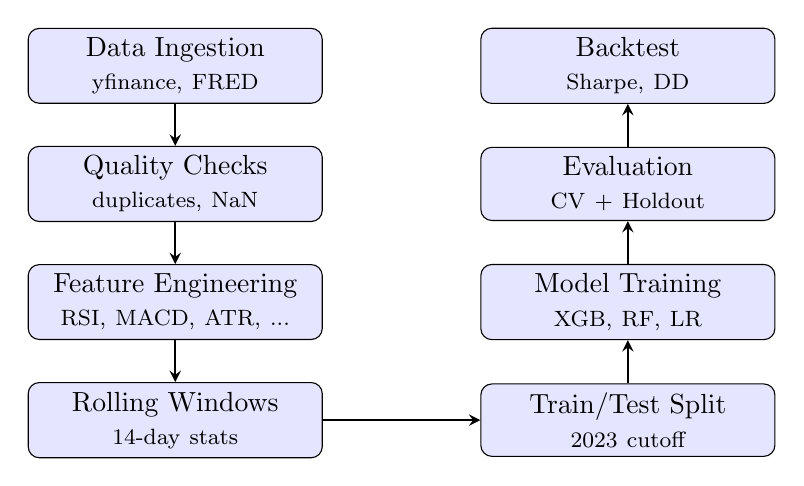
\begin{tikzpicture}[
            node distance=1.5cm,
            box/.style={rectangle, draw, fill=blue!10, text width=3.5cm, text centered, rounded corners, minimum height=0.8cm},
            arrow/.style={->, >=stealth, thick}
        ]
            \node[box] (data) {Data Ingestion\\{\footnotesize yfinance, FRED}};
            \node[box, below of=data] (quality) {Quality Checks\\{\footnotesize duplicates, NaN}};
            \node[box, below of=quality] (features) {Feature Engineering\\{\footnotesize RSI, MACD, ATR, ...}};
            \node[box, below of=features] (rolling) {Rolling Windows\\{\footnotesize 14-day stats}};
            \node[box, right=2cm of rolling] (split) {Train/Test Split\\{\footnotesize 2023 cutoff}};
            \node[box, above of=split] (models) {Model Training\\{\footnotesize XGB, RF, LR}};
            \node[box, above of=models] (eval) {Evaluation\\{\footnotesize CV + Holdout}};
            \node[box, above of=eval] (backtest) {Backtest\\{\footnotesize Sharpe, DD}};

            \draw[arrow] (data) -- (quality);
            \draw[arrow] (quality) -- (features);
            \draw[arrow] (features) -- (rolling);
            \draw[arrow] (rolling) -- (split);
            \draw[arrow] (split) -- (models);
            \draw[arrow] (models) -- (eval);
            \draw[arrow] (eval) -- (backtest);
        \end{tikzpicture}
    \end{center}
\end{frame}

\begin{frame}[fragile]{Key Implementation Details}
    \textbf{Libraries Used:}
    \begin{itemize}
        \item \textbf{Data:} \texttt{pandas}, \texttt{numpy}, \texttt{yfinance}
        \item \textbf{ML:} \texttt{scikit-learn}, \texttt{xgboost}
        \item \textbf{Technical Analysis:} \texttt{ta}
        \item \textbf{Visualization:} \texttt{plotly}, \texttt{seaborn}, \texttt{matplotlib}
    \end{itemize}

    \vspace{0.3cm}

    \textbf{Reproducibility:}
    \begin{lstlisting}[language=Python]
SEED = 42
np.random.seed(SEED)
# All models use random_state=SEED
# Chronological split at 2023-01-01
# Fixed hyperparameters documented
    \end{lstlisting}

    \vspace{0.3cm}

    \textbf{Code Structure:}
    \begin{itemize}
        \item Modular functions for data loading, feature engineering, training
        \item Self-contained Jupyter notebook for transparency
        \item All steps executable top-to-bottom
    \end{itemize}
\end{frame}

% Section 7: Training and Evaluation
\section{Training and Evaluation}

\begin{frame}{Data Splitting Strategy}
    \textbf{Chronological Split (Temporal Validation):}
    \begin{itemize}
        \item \textbf{Training:} All data before 2023-01-01 (2,038 samples)
        \item \textbf{Test:} All data from 2023-01-01 onward (2,319 samples)
        \item \textbf{Rationale:} Prevents data leakage, mimics real deployment
    \end{itemize}

    \vspace{0.3cm}

    \textbf{Cross-Validation:}
    \begin{itemize}
        \item 5-fold TimeSeriesSplit on training data
        \item Each fold uses only past data for training
        \item Metric: Precision (emphasis on avoiding false positives)
    \end{itemize}

    \vspace{0.3cm}

    \textbf{Evaluation Metrics:}
    \begin{itemize}
        \item \textbf{ML Metrics:} Precision, Recall, F1, ROC-AUC, PR-AUC
        \item \textbf{Strategy Metrics:} Annualized return, Sharpe ratio, Max drawdown
    \end{itemize}
\end{frame}

\begin{frame}{Model Hyperparameters}
    \begin{table}
        \centering
        \small
        \begin{tabular}{lp{7cm}}
            \toprule
            \textbf{Model} & \textbf{Key Hyperparameters} \\
            \midrule
            XGBoost & n\_estimators=300, max\_depth=4, lr=0.05, subsample=0.9, colsample=0.9, scale\_pos\_weight=2.15 \\
            \midrule
            Random Forest & n\_estimators=400, max\_depth=8, min\_samples\_leaf=8, class\_weight='balanced\_subsample' \\
            \midrule
            Logistic Reg. & solver='liblinear', class\_weight='balanced', max\_iter=4000 \\
            \bottomrule
        \end{tabular}
    \end{table}

    \vspace{0.3cm}

    \textbf{Class Balancing:}
    \begin{itemize}
        \item Positive class: 34.3\% → \texttt{scale\_pos\_weight} = 1.92
        \item Ensures model doesn't ignore minority class
    \end{itemize}
\end{frame}

\begin{frame}{Cross-Validation Results}
    \textbf{XGBoost Time-Series CV (5 folds):}

    \begin{table}
        \centering
        \begin{tabular}{cc}
            \toprule
            \textbf{Fold} & \textbf{Precision} \\
            \midrule
            1 & 0.4561 \\
            2 & 0.3333 \\
            3 & 0.1000 \\
            4 & 0.6667 \\
            5 & 0.2708 \\
            \midrule
            \textbf{Best} & \textbf{0.6667} \\
            \bottomrule
        \end{tabular}
    \end{table}

    \vspace{0.3cm}

    \textbf{Observations:}
    \begin{itemize}
        \item High variance across folds (expected for volatile stocks)
        \item Fold 4 shows best precision (66.7\%)
        \item Indicates sensitivity to market regime
    \end{itemize}
\end{frame}

% Section 8: Results
\section{Results and Discussion}

\begin{frame}{Final Model Performance}
    \textbf{Test Set Results (2023+):}

    \begin{table}
        \centering
        \begin{tabular}{lcccc}
            \toprule
            \textbf{Model} & \textbf{Precision} & \textbf{Recall} & \textbf{F1} & \textbf{ROC-AUC} \\
            \midrule
            XGBoost & 0.366 & 0.380 & 0.373 & \textbf{0.513} \\
            Random Forest & 0.390 & 0.247 & 0.303 & 0.518 \\
            Logistic Reg. & 0.399 & 0.413 & 0.406 & 0.506 \\
            \bottomrule
        \end{tabular}
    \end{table}

    \vspace{0.3cm}

    \textbf{Overall Performance:}
    \begin{itemize}
        \item \textbf{Accuracy:} 53-58\% (slightly better than random 50\%)
        \item \textbf{ROC-AUC:} 0.51-0.52 (weak signal)
        \item \textbf{Best model:} Random Forest (by precision) or XGBoost (by AUC)
    \end{itemize}

    \vspace{0.3cm}

    \begin{alertblock}{Reality Check}
        Stock prediction is inherently difficult. These results are \textbf{realistic} for technical analysis-based models.
    \end{alertblock}
\end{frame}

\begin{frame}{Threshold Tuning}
    \textbf{Impact of Decision Threshold:}

    \begin{itemize}
        \item Default threshold: 0.50
        \item Tested range: 0.30 to 0.85
        \item \textbf{Trade-off:} Higher threshold → better precision, lower recall
    \end{itemize}

    \vspace{0.3cm}

    \textbf{Strategy-Level Evaluation:}
    \begin{itemize}
        \item Best Sharpe ratio at threshold = 0.30
        \item Annualized return: 31.3\%
        \item Sharpe: 0.886
        \item Max drawdown: -28.4\%
    \end{itemize}

    \vspace{0.3cm}

    \begin{block}{Key Insight}
        Lower thresholds generate more trades (higher coverage) but with less precision. Choice depends on risk appetite.
    \end{block}
\end{frame}

\begin{frame}{Strengths and Weaknesses}
    \begin{columns}
        \column{0.5\textwidth}
        \textbf{Strengths:}
        \begin{itemize}
            \item \cmark{} Strict chronological validation
            \item \cmark{} Multiple models compared
            \item \cmark{} Clean, interpretable features
            \item \cmark{} Threshold tuning
            \item \cmark{} Feature ablation
            \item \cmark{} Honest performance assessment
        \end{itemize}

        \column{0.5\textwidth}
        \textbf{Weaknesses:}
        \begin{itemize}
            \item \xmark{} Low predictive power (~51\% AUC)
            \item \xmark{} High-volatility stocks hard to predict
            \item \xmark{} No transaction costs modeled
            \item \xmark{} Market regime dependent
            \item \xmark{} No probability calibration
            \item \xmark{} Limited to technical features
        \end{itemize}
    \end{columns}

    \vspace{0.5cm}

    \textbf{Practical Implications:}
    \begin{itemize}
        \item Model works as \textbf{decision support}, not standalone system
        \item Should be combined with fundamental analysis
        \item Requires active risk management
    \end{itemize}
\end{frame}

\begin{frame}{Why is Performance Limited?}
    \textbf{Efficient Market Hypothesis:}
    \begin{itemize}
        \item Prices already reflect available information
        \item Technical patterns are weak predictors
        \item News and sentiment drive volatile stocks more than charts
    \end{itemize}

    \vspace{0.3cm}

    \textbf{Challenges Specific to High-Volatility Stocks:}
    \begin{enumerate}
        \item \textbf{Unpredictable catalysts:} Earnings surprises, FDA approvals, government contracts
        \item \textbf{Social media influence:} Reddit/Twitter can move prices rapidly
        \item \textbf{Low liquidity events:} Flash crashes and squeezes
        \item \textbf{Regime shifts:} Bull/bear transitions change patterns
    \end{enumerate}

    \vspace{0.3cm}

    \begin{block}{Academic Insight}
        Our results (53\% accuracy, 0.51 AUC) are \textbf{typical} for academic research on stock prediction using technical analysis alone
    \end{block}
\end{frame}

% Section 9: Conclusion
\section{Conclusion}

\begin{frame}{Key Achievements}
    \textbf{What we accomplished:}

    \begin{enumerate}
        \item \cmark{} Built end-to-end ML pipeline for stock prediction
        \item \cmark{} Rigorous temporal validation (no data leakage)
        \item \cmark{} Comprehensive feature engineering (technical + macro)
        \item \cmark{} Multiple model comparison (XGB, RF, LR)
        \item \cmark{} Dual evaluation (ML metrics + strategy backtest)
        \item \cmark{} Threshold optimization
        \item \cmark{} Feature ablation study
        \item \cmark{} Honest assessment of limitations
    \end{enumerate}

    \vspace{0.3cm}

    \textbf{Lessons Learned:}
    \begin{itemize}
        \item Stock prediction is much harder than typical ML classification
        \item More features $\neq$ better performance (simplicity matters)
        \item Threshold choice critical for trading applications
        \item Backtesting reveals hidden issues ML metrics miss
    \end{itemize}
\end{frame}

\begin{frame}{Overall Impact and Value}
    \textbf{Educational Value:}
    \begin{itemize}
        \item Realistic case study of ML in finance
        \item Understanding when ML works and when it doesn't
        \item Importance of domain knowledge
        \item Critical evaluation of results
    \end{itemize}

    \vspace{0.3cm}

    \textbf{Technical Skills Gained:}
    \begin{itemize}
        \item Time-series ML workflow
        \item Feature engineering for financial data
        \item Model selection and hyperparameter tuning
        \item Backtesting and risk metrics
        \item Data visualization and communication
    \end{itemize}

    \vspace{0.3cm}

    \begin{block}{Key Takeaway}
        ML can provide \textbf{marginal edge} in financial markets, but is not a "magic solution". Success requires combining ML with domain expertise, risk management, and realistic expectations.
    \end{block}
\end{frame}

% Section 10: Future Work
\section{Future Work}

\begin{frame}{Possible Improvements}
    \textbf{Short-term Enhancements:}
    \begin{enumerate}
        \item Add transaction costs and slippage to backtest
        \item Implement probability calibration (Platt scaling)
        \item Try ensemble methods (stacking, voting)
        \item Add more alternative data sources
    \end{enumerate}

    \vspace{0.3cm}

    \textbf{Advanced Features to Explore:}
    \begin{itemize}
        \item \textbf{Sentiment analysis:} News headlines, social media
        \item \textbf{Options data:} Implied volatility, put/call ratios
        \item \textbf{Fundamental data:} Earnings, revenue growth
        \item \textbf{Intraday patterns:} Opening gaps, VWAP
    \end{itemize}

    \vspace{0.3cm}

    \textbf{Model Improvements:}
    \begin{itemize}
        \item Deep learning (LSTM, Transformers for time-series)
        \item Reinforcement learning for trading policy
        \item Multi-task learning (predict multiple horizons)
    \end{itemize}
\end{frame}

\begin{frame}{Deployment Considerations}
    \textbf{Real-World Deployment Path:}

    \begin{enumerate}
        \item \textbf{Walk-forward validation:} Retrain model monthly/quarterly
        \item \textbf{Monitoring system:} Track model drift, feature distributions
        \item \textbf{Risk controls:} Position sizing, stop-losses, portfolio limits
        \item \textbf{Paper trading:} Test in simulation before real capital
        \item \textbf{Incremental rollout:} Start with small capital allocation
    \end{enumerate}

    \vspace{0.3cm}

    \textbf{Scaling Opportunities:}
    \begin{itemize}
        \item Expand to more volatile stocks
        \item Multi-asset portfolio optimization
        \item Regime-switching models
        \item Integration with existing trading platforms
    \end{itemize}

    \vspace{0.3cm}

    \begin{alertblock}{Caution}
        Real deployment requires regulatory compliance, proper risk management, and continuous monitoring
    \end{alertblock}
\end{frame}

% Appendices
\section{Appendices}

\begin{frame}{Configuration Details}
    \textbf{Environment Setup:}
    \begin{itemize}
        \item Python 3.11
        \item Key libraries: pandas 2.0+, scikit-learn 1.3+, xgboost 2.0+
        \item Random seed: 42 (all experiments)
    \end{itemize}

    \vspace{0.3cm}

    \textbf{Model Parameters:}

    \begin{table}
        \centering
        \footnotesize
        \begin{tabular}{ll}
            \toprule
            \textbf{Parameter} & \textbf{Value} \\
            \midrule
            Horizon (days) & 5 \\
            Success threshold & 3.5\% \\
            Rolling window & 14 days \\
            Train/test cutoff & 2023-01-01 \\
            CV folds & 5 (TimeSeriesSplit) \\
            \bottomrule
        \end{tabular}
    \end{table}
\end{frame}

\begin{frame}{Feature Importance (XGBoost)}
    \textbf{Top 10 Most Important Features:}

    \begin{enumerate}
        \item \texttt{atr\_14\_mean} - ATR rolling mean (volatility)
        \item \texttt{rsi\_14\_last} - Most recent RSI value
        \item \texttt{ten\_year\_yield\_mean} - Macro factor average
        \item \texttt{macd\_hist\_std} - MACD histogram variability
        \item \texttt{volume\_z\_last} - Recent volume anomaly
        \item \texttt{bb\_width\_std} - Bollinger Band width variability
        \item \texttt{ma\_50\_mean} - 50-day MA rolling average
        \item \texttt{atr\_pct\_std} - ATR percentage variability
        \item \texttt{macd\_signal\_mean} - MACD signal average
        \item \texttt{rsi\_14\_mean} - RSI rolling average
    \end{enumerate}

    \vspace{0.2cm}

    \textbf{Insight:} ATR and volatility features dominate, confirming their importance for high-volatility regime
\end{frame}

\begin{frame}[plain]
    \begin{center}
        \Huge \textbf{Thank You!}

        \vspace{1.5cm}

        \LARGE Questions?

        \vspace{1.5cm}

        \large
        \textbf{Contact:}\\
        \vspace{0.3cm}
        Dalil ADIMI \& Hassen BEN AMOR\\
        Group I2-NEW DAI\\
        EFREI Paris
    \end{center}
\end{frame}

\end{document}
